\documentclass[12pt]{article}
\usepackage[top=1in, bottom=1in, left=1in, right=1in]{geometry}

\usepackage{setspace}
\onehalfspacing

\usepackage{amssymb}
%% The amsthm package provides extended theorem environments
\usepackage{amsthm}
\usepackage{epsfig}
\usepackage{times}
\renewcommand{\ttdefault}{cmtt}
\usepackage{amsmath}
\usepackage{graphicx} % for graphics files
\usepackage{tabu}

% Draw figures yourself
\usepackage{tikz} 

% writing elements
\usepackage{mhchem}

% The float package HAS to load before hyperref
\usepackage{float} % for psuedocode formatting
\usepackage{xspace}

% from Denovo Methods Manual
\usepackage{mathrsfs}
\usepackage[mathcal]{euscript}
\usepackage{color}
\usepackage{array}

\usepackage[pdftex]{hyperref}
\usepackage[parfill]{parskip}

% math syntax
\newcommand{\nth}{n\ensuremath{^{\text{th}}} }
\newcommand{\ve}[1]{\ensuremath{\mathbf{#1}}}
\newcommand{\Macro}{\ensuremath{\Sigma}}
\newcommand{\rvec}{\ensuremath{\vec{r}}}
\newcommand{\vecr}{\ensuremath{\vec{r}}}
\newcommand{\omvec}{\ensuremath{\hat{\Omega}}}
\newcommand{\vOmega}{\ensuremath{\hat{\Omega}}}
\newcommand{\sigs}{\ensuremath{\Sigma_s(\rvec,E'\rightarrow E,\omvec'\rightarrow\omvec)}}
\newcommand{\el}{\ensuremath{\ell}}
\newcommand{\sigso}{\ensuremath{\Sigma_{s,0}}}
\newcommand{\sigsi}{\ensuremath{\Sigma_{s,1}}}
%---------------------------------------------------------------------------
%---------------------------------------------------------------------------
\begin{document}
\begin{center}
{\bf NE 250, F15\\
November 2, 2015 
}
\end{center}

We've derived the Transport Equation, from it derived the Diffusion Equation, talked about the TE in the integral form, looked at the adjoint in detail, and quickly covered Monte Carlo methods. Finally, what about solving the integro-differential TE itself? That's next. We start with

The \textbf{Multigroup Approximation} (from L\&M 2.2)\\
We begin by setting up an energy grid, where $E_0$ is the highest energy value and $E_G$ is the lowest. We get $G-1$ groups and call the group between edge $g$ and edge $g-1$ group $g$. 

\begin{center}
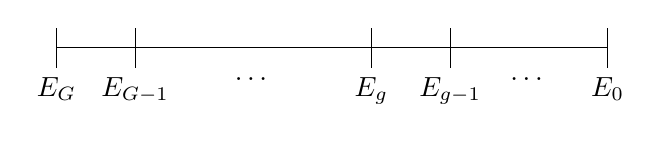
\begin{tikzpicture}
\draw (0,0)--(7,0);
\draw (0,-0.25)--(0, 0.25);
\draw (1,-0.25)--(1, 0.25);
\draw (4,-0.25)--(4, 0.25);
\draw (5,-0.25)--(5, 0.25);
\draw (7,-0.25)--(7, 0.25);
\node[below] at (0,-.25) {$E_G$};
\node[below] at (1,-.25) {$E_{G-1}$};
\node[below] at (2.5,-.25) {$\dots$};
\node[below] at (4,-.25) {$E_g$};
\node[below] at (5,-.25) {$E_{g-1}$};
\node[below] at (6,-.25) {$\dots$};
\node[below] at (7,-.25) {$E_0$};
\end{tikzpicture}
\end{center}

We use this grid to define the group flux
\[
\psi_g(\vecr, \vOmega) \equiv \int_{E_g}^{E_{g-1}} dE\: \psi(\vecr, \vOmega, E)
\]
Note that the continuous $\psi$ is in units of per eV, while the group angular flux is not, it includes all of the neutrons over that energy group. What we want to do next, is derive an equation whose solution is $\psi_g$, which means we will integrate the entire TE over energy. 

To perform that integral, we need to introduce an approximation. The one we will talk about now is \textit{assume the angular flux is separable in energy}:
\[
\psi(\vec{r}, \vOmega, E) \approx f(E)\psi_g(\vec{r}, \vOmega)\:, \quad E_g < E \leq E_{g-1}\:,
\]
where $f(E)$ is normalized such that $\int_g dE\: f(E) = 1$ (note that this means $f$ has units of per eV). We substitute and/or use this in the regular TE and integrate over energy. Here's how that works term by term.
%
\begin{itemize}
\item Streaming:
\[
\int_{E_g}^{E_{g-1}} dE\: \vOmega \cdot \nabla \psi(\vec{r}, \vOmega, E) = \int_{E_g}^{E_{g-1}} dE\: \vOmega \cdot \nabla f(E)\psi_g(\vec{r}, \vOmega) = \vOmega \cdot \nabla \psi_g(\vec{r}, \vOmega)
\]

\item External (distributed fixed) source:
\[q_{g}(\vec{r}, \vOmega) \equiv \int_{E_g}^{E_{g-1}} dE\: q(\vec{r}, \vOmega, E)\]

\item Fission Source:
\begin{align*}
\int_{E_g}^{E_{g-1}} dE\: &\frac{\chi(E)}{4 \pi}\int_0^{\infty} dE' \: \nu(E') \Sigma_f(E') \int_{4 \pi} d\vOmega' \:\psi(\vec{r}, E', \vOmega') \\
&\chi_g \equiv \int_{E_g}^{E_{g-1}} dE\: \chi(E) \\
& \int_{4 \pi} d\vOmega' \:\psi_g(\vec{r}, \vOmega') = \phi_g(\vec{r})\\
& \int_0^{\infty} dE' \: \nu(E') \Sigma_f(E') = \sum_{g'=1}^G \int_{E_g'}^{E_{g'-1}} dE'\: \nu(E') \Sigma_f(E')
\end{align*}
These second two items combine to form the fission source from group $g'$. We also need to define
\[
\nu\Sigma_{fg'} = \int_{E_g'}^{E_{g'-1}} dE'\: \nu(E') \Sigma_f(E') f(E')
\]
and therefore the fission source in group $g$ is
\[
q_{fg} = \frac{\chi_g}{4 \pi}\sum_{g'=1}^G \nu\Sigma_{fg'} \phi_{g'}(\vec{r})
\]

\item Scattering term:
\[
q_{s,gg'}(\vOmega) \equiv \int_{E_g}^{E_{g-1}} dE \int_{E_g'}^{E_{g'-1}} dE' \int_{4 \pi} d\vOmega' \: \Sigma_s(E'\rightarrow E, \vOmega' \cdot \vOmega) \psi(\vec{r}, E', \vOmega')
\]
If we generically define the scattering cross section this we, we can get this general scattering expression
\begin{align*}
\Sigma_{s,gg'}(\vOmega' \cdot \vOmega) & \equiv \int_{E_g}^{E_{g-1}} dE \int_{E_g'}^{E_{g'-1}} dE' \: \Sigma_s(E'\rightarrow E, \vOmega' \cdot \vOmega) f(E')\\
q_{s,g}(\vOmega) &= \sum_{g'=1}^G \int_{4 \pi} d\vOmega' \Sigma_{s,gg'}(\vOmega' \cdot \vOmega) \psi_{g'}(\vec{r}, \vOmega')
\end{align*}

\item Total interaction:
\begin{align*}
\Sigma_{tg}(\vec{r}) &= \int_{E_g}^{E_{g-1}} dE\: \Sigma_t(\vec{r}, E)f(E)\\
\text{term }&= \Sigma_{tg} \psi_g(\vec{r}, \vOmega)
\end{align*}

\end{itemize}
%
We can combine all of this to get a conventional, general expression for the \textbf{multigroup TE}.
\begin{align*}
[\vOmega \cdot \nabla + \Sigma_{tg}(\vec{r})]\psi_g(\vec{r}, \vOmega) =&  \sum_{g'=1}^G \int_{4 \pi} d\vOmega'\: \Sigma_{s,gg'}(\vecr, \vOmega' \cdot \vOmega) \psi_{g'}(\vec{r}, \vOmega')\\
&+\frac{\chi_g}{4 \pi}\sum_{g'=1}^G \nu\Sigma_{fg'}(\vec{r}) \phi_{g'}(\vec{r}) + q_g(\vec{r}, \vOmega)
\end{align*}
If we want, we can integrate this equation over angle to get a balance equation and from there derive the multigroup diffusion equation.

---------------------------------\\
\textbf{Group Constants}\\
To solve this equation, we need all of the collapsed cross section values to come from somewhere (for this to be accurate, we need the detailed energy dependence of the cross sections and the spectral weighting function, $f(E)$, to be known). 

For smoothly varying parts of the cross section, it is reasonable easy to make weighting function assumptions. However, in resonance regions even very fine group structures are insufficient and we get self-shielding effects that will be missed. There are a variety of methods to attempt to capture this behavior, but we will not go into them here.

In a general sense, we often 
\begin{enumerate}
\item start with ENDF data (1000s of energy groups), and then do an infinite medium or 1-D transport calculation and use the results to collapse the data to 100s of energy groups.

\item Following this we often do another transport calculation at the level of a unit cell or assembly and then collapse in energy and homogenize in space, getting us few to 10s of groups.\\
We will take, e.g.\ an assembly from the middle of the core and put reflecting boundary conditions on all sides and solve for either $\psi_g(\vec{r}, \vOmega)$ or $\phi_{l,g}^m(\vec{r})$ (see below) to use in the collapsing.

\item Finally, we do a core level calculation with diffusion theory. 
\end{enumerate}

Collapsing in energy with fine groups (indexed $j$) into coarse group (indexed $h$):
\[
\Sigma_{h} \equiv \frac{\sum_{j \in h} \Sigma_{j} \phi_j(\vec{r})}{\sum_{j\in h} \phi_j(\vec{r})}
\]
and you would replace $\phi_g$ with $\psi_g$ or $\phi_{l,g}^m$ if doing scattering. 

Homogenizing in space (flux-weighting):
\[
\Sigma_j^{homog} \equiv \frac{\int_V dV \: \Sigma_j(\vec{r}) \phi_g(\vec{r})}{\int_V dV \: 
\phi_g(\vec{r})}
\]
where $V$ is a region made up of different nuclides at each point. 





\end{document}
